% COMPILE: xelatex

\documentclass[a4paper]{article}  % A4 paper size

\usepackage[UTF8]{ctex}  % Chinese support
\usepackage[left=3.17cm, right=3.17cm, top=2.54cm, bottom=2.54cm]{geometry}  % Margins

\usepackage{xcolor}  % Color support
\usepackage{tcolorbox}  % Colored boxes

\usepackage{fancyhdr}  % Header and footer
\usepackage{graphicx, subcaption}  % Figures
\usepackage[shortlabels]{enumitem}  % Enumerate list
\usepackage[sort&compress]{gbt7714}  % Bibliography
\usepackage{hyperref}  % Hyperlinks
\usepackage{booktabs, array}  % Tables
\usepackage{multirow}  % Multirow
\usepackage{amsmath}  % Math

\tcbuselibrary{skins}  % Colored boxes
\tcbuselibrary{minted}  % Code blocks

\setmonofont[]{Fira Code}  % Monospaced font
\usemintedstyle{colorful}  % Code block style set up
\setenumerate{  % Enumerate list set up
    itemsep=0pt,
    partopsep=0pt,
    parsep=\parskip,
    topsep=0pt,
    itemindent=4em,
    leftmargin=0pt,
    listparindent=2em,
    label= (\arabic*)
}
\setitemize{  % Itemize list set up
    itemsep=0pt,
    partopsep=0pt,
    parsep=\parskip,
    topsep=5pt
}
\setdescription{  % Description list set up
    itemsep=0pt,
    partopsep=0pt,
    parsep=\parskip,
    topsep=5pt
}
\hypersetup{  % Hyperlinks set up
    unicode,
    colorlinks=true,
    linkcolor=black,
    urlcolor=black
}



\newtcblisting{codeblock}[2][]{
    listing engine=minted,
    boxrule=0.1mm,
    colback=white!98!black,
    colframe=white!80!black,
    listing only,
    left=5mm,
    enhanced,
    sharp corners=all,
    overlay={
        \begin{tcbclipinterior}
            \fill[white!98!black] (frame.south west) rectangle ([xshift=5mm]frame.north west);
        \end{tcbclipinterior}
    },
    minted language=#2,
    minted style=tango,
    minted options={fontsize=\small,breaklines,autogobble,linenos,numbersep=3mm,escapeinside=\#\#},#1  % Use \# as escape character
}


\begin{document}

\title{\textbf{语音合成}\\Matlab 大作业报告}  % Title
\author{陈子熠}
\date{\today}
\maketitle

\tableofcontents

\newpage

\section{语音预测模型}

\subsection{}

给定
\begin{align*}
    e(n) &= s(n) - a_1s(n-1) - a_2s(n-2) \\
\end{align*}

假设 $e(n)$ 是输入信号,$s(n)$ 是输出信号,等式两边同时取 Z 变换,得上述滤波器的传递函数:
\begin{align*}
    H(z) &= \frac{S(z)}{E(z)} = \frac{1}{1 - a_1z^{-1} - a_2z^{-2}}
\end{align*}

如果 $a_1 = 1.3789,\ a_2 = −0.9506$ ,极点幅角:
\begin{codeblock}{matlab}
    a1 = 1.3789;
    a2 = -0.9506;
    b = 1;
    a = [1, -a1, -a2];
    sys = tf(b, a);
    p = pole(sys);
    angle(p)
\end{codeblock}
得:
\begin{align*}
    \Omega &= 0.7854
\end{align*}

正规化共振峰频率:
\begin{align*}
    f &= \Omega / \pi\ (\times \pi\ \text{rad/sample}) = 0.25\ (\times \pi\ \text{rad/sample})
\end{align*}

用 zplane 绘制零极点图:
\begin{codeblock}
    z = zero(sys);
    zplane(z, p);
\end{codeblock}
零极点图如图 \ref{fig:zplane}。

用 freqz 绘制频率响应:
\begin{codeblock}{matlab}
    freqz(b, a);
\end{codeblock}
频率响应如图 \ref{fig:freqz}。

用 impz 绘制单位样值响应:
\begin{codeblock}{matlab}
    impz(b, a, 200);
\end{codeblock}
单位样值响应如图 \ref{fig:impz}。

用 filter 绘制单位样值响应:
\begin{codeblock}{matlab}
    x = [1, zeros(1, 199)];
    y = filter(b, a, x);
    figure;
    plot(y);
    xlabel('n (samples)');
    ylabel('Amplitude');
    title('Impulse Response of using Filter');
\end{codeblock}
单位样值响应如图 \ref{fig:filter}。

\begin{figure}[ht]
    \centering
    \begin{subfigure}[b]{0.48\textwidth}
        \centering
        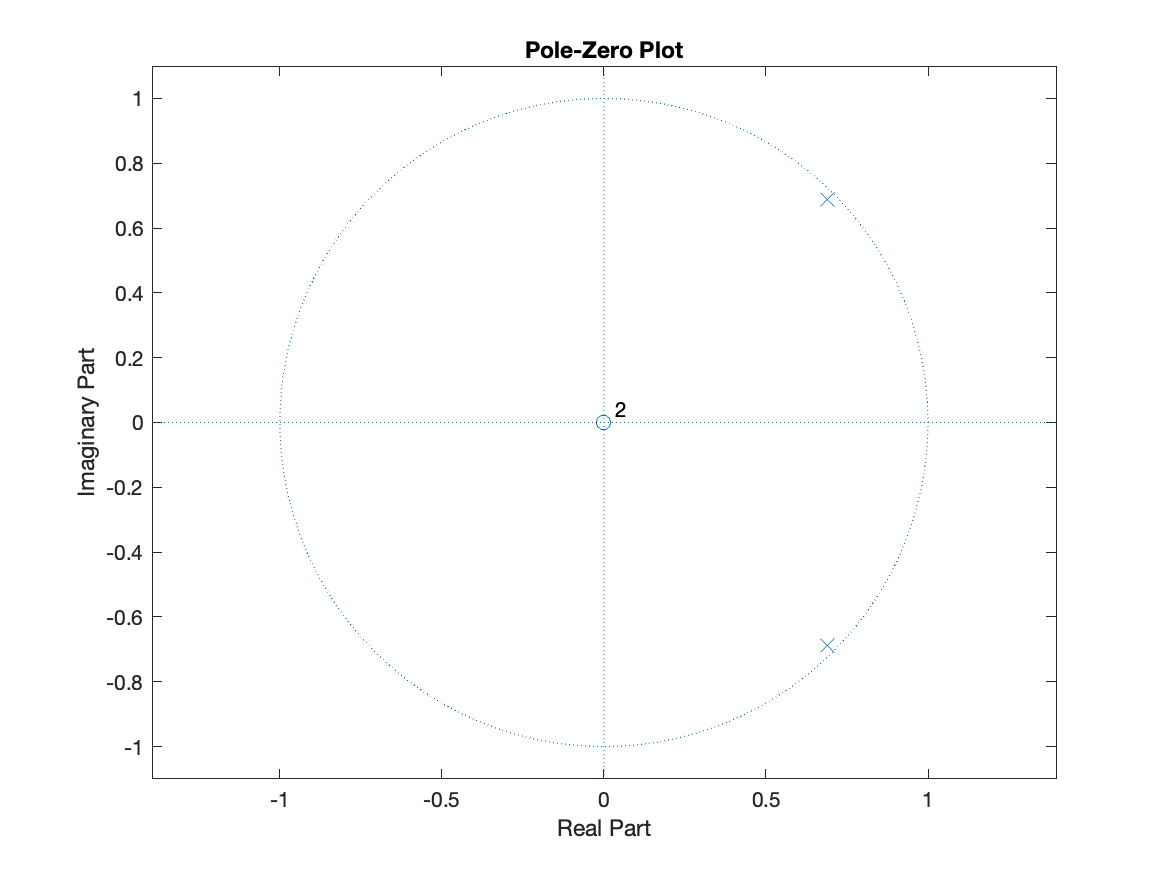
\includegraphics[width=\textwidth]{asserts/1_1_zplane.png}
        \caption{
            用 zplane 绘制的零极点图
        }\label{fig:zplane}
    \end{subfigure}
    \hfill
    \begin{subfigure}[b]{0.48\textwidth}
        \centering
        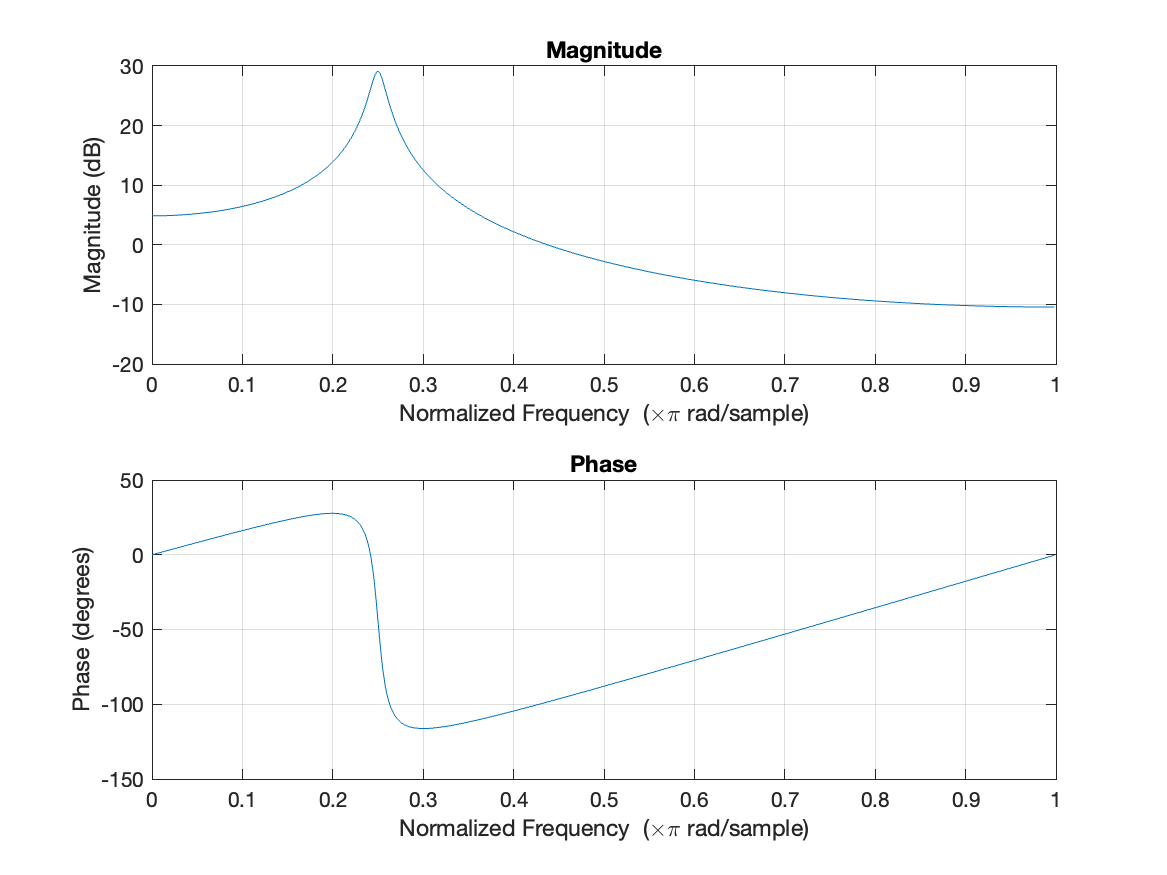
\includegraphics[width=\textwidth]{asserts/1_1_freqz.png}
        \caption{
            用 freqz 绘制的频率响应
        }\label{fig:freqz}
    \end{subfigure}
    \caption{
        零极点图与频率响应
    }
\end{figure}

\begin{figure}[ht]
    \begin{subfigure}[b]{0.48\textwidth}
        \centering
        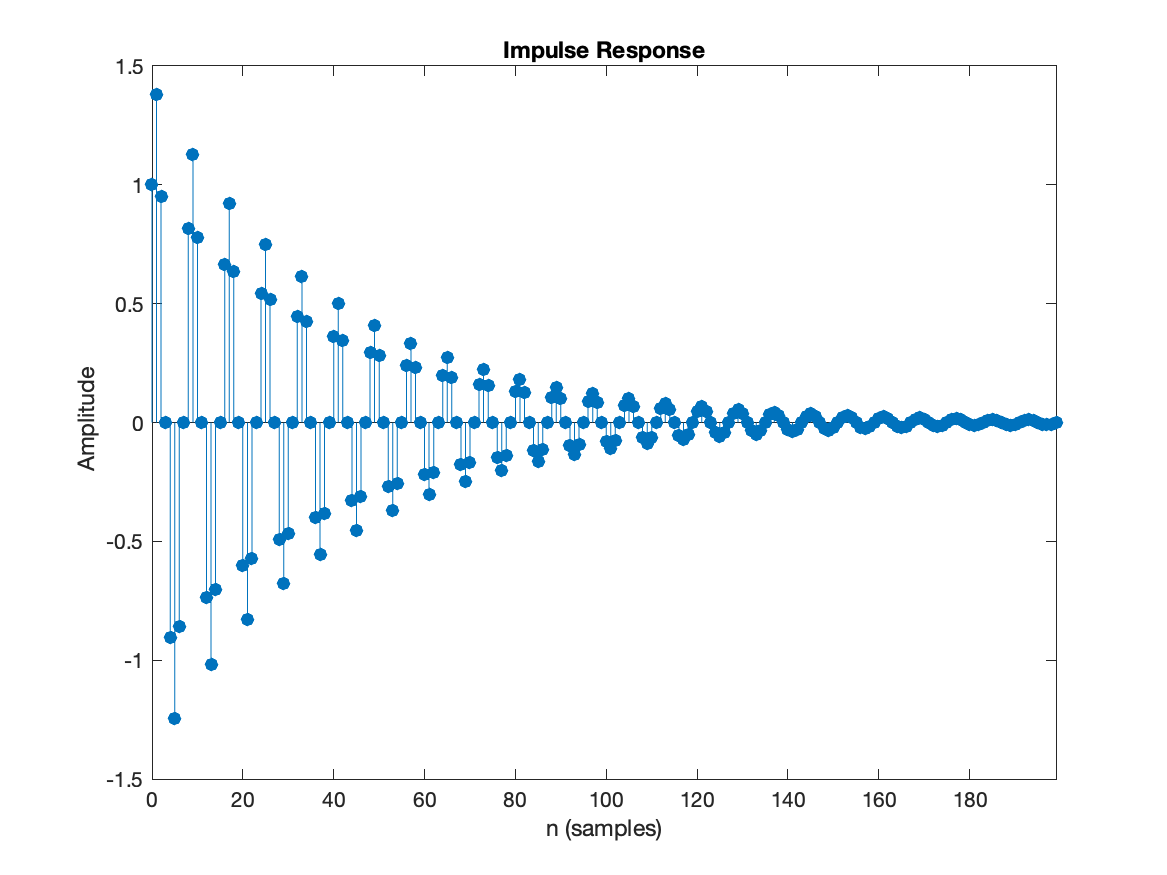
\includegraphics[width=\textwidth]{asserts/1_1_impz.png}
        \caption{
            用 impz 绘制的单位样值响应
        }\label{fig:impz}
    \end{subfigure}
    \hfill
    \begin{subfigure}[b]{0.48\textwidth}
        \centering
        \includegraphics[width=\textwidth]{asserts/1_1_filter.png}
        \caption{
            用 filter 绘制的单位样值响应
        }\label{fig:filter}
    \end{subfigure}
    \caption{
        单位样值响应
    }
\end{figure}

\section{语音合成模型}
\section{变速不变调}
\section{变调不变速}


% % HEADER AND FOOTER
% \pagestyle{fancy}
% \fancyhf{}
% \lhead{LEFT HEADER}
% \chead{CENTER HEADER}
% \rhead{RIGHT HEADER}
% \lfoot{LEFT FOOTER}
% \cfoot{CENTER FOOTER}
% \rfoot{RIGHT FOOTER}
% \renewcommand{\headrulewidth}{0.4pt}
% \renewcommand{\footrulewidth}{0.4pt}

% % ABSTRACT
% \begin{abstract}
%     ABSTRACT
% \end{abstract}

% % SECTION
% \section{SECTION}\label{sec:LABEL}
% \subsection{subsection}
% \subsubsection{subsubsection}

% % TEXT
% PLAIN
% \textbf{BOLD}
% \textit{ITALIC}
% \underline{UNDERLINE}
% \textcolor{red}{RED}
% \href{https://www.eesast.com}{HYPERLINK}

% % REFERENCE
% ref to section\ref{sec:LABEL}
% ref to figure\ref{fig:LABEL}
% ref to table\ref{tab:LABEL}
% ref to appendix\ref{adx:ASM}
% ref to citation\cite{REF}

% % FIGURE
% \begin{figure}[ht]  % h: here, t: top, b: bottom, p: page
%     \centering
%     \includegraphics[width=.8\textwidth]{FIG.png}  % Width: 0.8 times of text width
%     \caption{CAPTION}\label{fig:FIGURE}
% \end{figure}

% % SUBFIGURE
% \begin{figure}[ht]
%     \centering
%     \begin{subfigure}[b]{0.48\textwidth}
%         \centering
%         \includegraphics[width=\textwidth]{FIG1.png}
%         \caption{
%             CAPTION1
%         }\label{fig:FIG1}
%     \end{subfigure}
%     \hfill
%     \begin{subfigure}[b]{0.48\textwidth}
%         \centering
%         \includegraphics[width=\textwidth]{FIG2.png}
%         \caption{
%             CAPTION2
%         }\label{fig:FIG2}
%     \end{subfigure}
%     \caption{
%         CAPTION1 \\
%         CAPTION2
%     }\label{fig:SUBFIGURE}
% \end{figure}

% % TABLE
% \begin{table}[htb]
%     \centering
%     \caption{CAPTION}\label{tab:LABEL}
%     \begin{tabular}{cc}  % c: center, l: left, r: right, p{2cm}: fixed width
%         \toprule
%         \textbf{HEADER1} & \textbf{HEADER2} \\
%         \midrule
%         CELL1 & CELL2 \\
%         CELL3 & CELL4 \\
%         CELL5 & CELL6 \\
%         \bottomrule
%     \end{tabular}
% \end{table}

% % CODE BLOCK
% \begin{codeblock}{ASM}
%     lw $v0, 114514($sp)
% \end{codeblock}

% % Enumerate list
% \begin{enumerate}[1]  % start from 1
%     % 1: Arabic number, a: Lowercase letter, A: Uppercase letter, i: Lowercase Roman numeral, I: Uppercase Roman numeral
%     \item ITEM1
%     \item ITEM2
%     \item ITEM3
% \end{enumerate}

% % Unreferenced literature
% \nocite{REF}
% \small{
%     \bibliographystyle{gbt7714-numerical}  % gbt7714-plain, gbt7714-numerical
%     \bibliography{ref}  % ref.bib
% }

% \newpage

% % Appendix
% \appendix
% \section{APPENDIX\label{adx:ASM}}


\end{document}